\documentclass[11pt, oneside]{article}   	% use "amsart" instead of "article" for AMSLaTeX format
\usepackage{geometry}                		% See geometry.pdf to learn the layout options. There are lots.
\geometry{letterpaper}                   		% ... or a4paper or a5paper or ... 
%\geometry{landscape}                		% Activate for rotated page geometry
%\usepackage[parfill]{parskip}    		% Activate to begin paragraphs with an empty line rather than an indent
\usepackage{graphicx}				% Use pdf, png, jpg, or eps§ with pdflatex; use eps in DVI mode
								% TeX will automatically convert eps --> pdf in pdflatex		
\usepackage{amssymb}
\usepackage{float}
%SetFonts

%SetFonts


\title{Bearings fault detection and classification with machine learning and signal processing}
\author{Yapi Donatien Achou}
%\date{}							% Activate to display a given date or no date

\begin{document}
\maketitle
\section{Introduction}
In this article I will describe two families of methods, to detect and identify different bearing fault type.
The first method uses statistical learning/method and the second methods uses signal processing.
In the statistical learning methods, we compute a statistical characteristics (mean, variance, kurtosis ...) of a reference sample
and use this measure to compute the dissimilarity between the reference sample and subsequent 
samples.\par
\begin{flushleft}
In the second method signal processing methods (Fast Fourier Transform) is used to extract the frequency spectrum of the vibration time signal of a bearing, and search for the bearing fault frequency. Once this fault frequency is identified , the corresponding 
amplitude is recorded and monitored for subsequent sample.
\end{flushleft}



\section{Bearing fault type}
When it comes to bearings, there are several fault type: Ball Pass Frequency Outer race defect (BPFO) which happen in the outer ring of the bearing, Ball Pass Frequency Inner race defect  (BPFI) which happen in the inner ring.

\begin{figure}[H] %  figure placement: here, top, bottom, or page
   \centering
   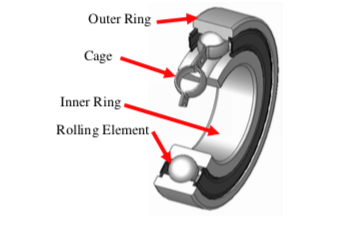
\includegraphics[width=4in]{bearing.png} 
   \caption{Geometrical representation of a ball bearing (Figure taken form [32])}
   \label{fig:bearing}
\end{figure}

\section{Dissimilarity measure}



\end{document}  